\chapter{Physical Network Design}

\section{Devices}
\subsection{CCTV}
\subsection{Wireless Access Points}
\subsection{Switches}
\subsection{Routers}
\subsection{}
\section{Wiring}
\subsection{Fibre}
\subsubsection{Multimode Fiber - OM4}
Could be used in and between core/access due to high data transfer rates (10Gbps) over a distance of 550m.\\
While the distance of 550m is overkill for a 7 story building, the allowance for higher distances at higher speeds (100m at 100Gbps) will be good for futurproofing our solution.\\
Use case would be from server room to server cupboard.\\
OM4 would be used due to the cost/benifit compared to OM5 which would be overkill for our setup.\\

\begin{table}[]
    \centering
    \begin{tabular}{|c|c|c|}
    \hline
    Type & Distance for a 10Gbps connection & Cost per meter \\ \hline
    OM1  & 33m                              &                \\ \hline
    OM2  & 82m                              &                \\ \hline
    OM3  & 300m                             &                \\ \hline
    OM4  & 550m                             &                \\ \hline
    OM5  & 550m                             &                \\ \hline
    \end{tabular}
\end{table}
\subsection{Copper - CAT6a}
Allows us to utilise 10Gbps over 100m. Use case would be from workstations to server cupboard.
\section{Device Placement}
\subsection{Ground Floor}
\begin{figure}[!h]
    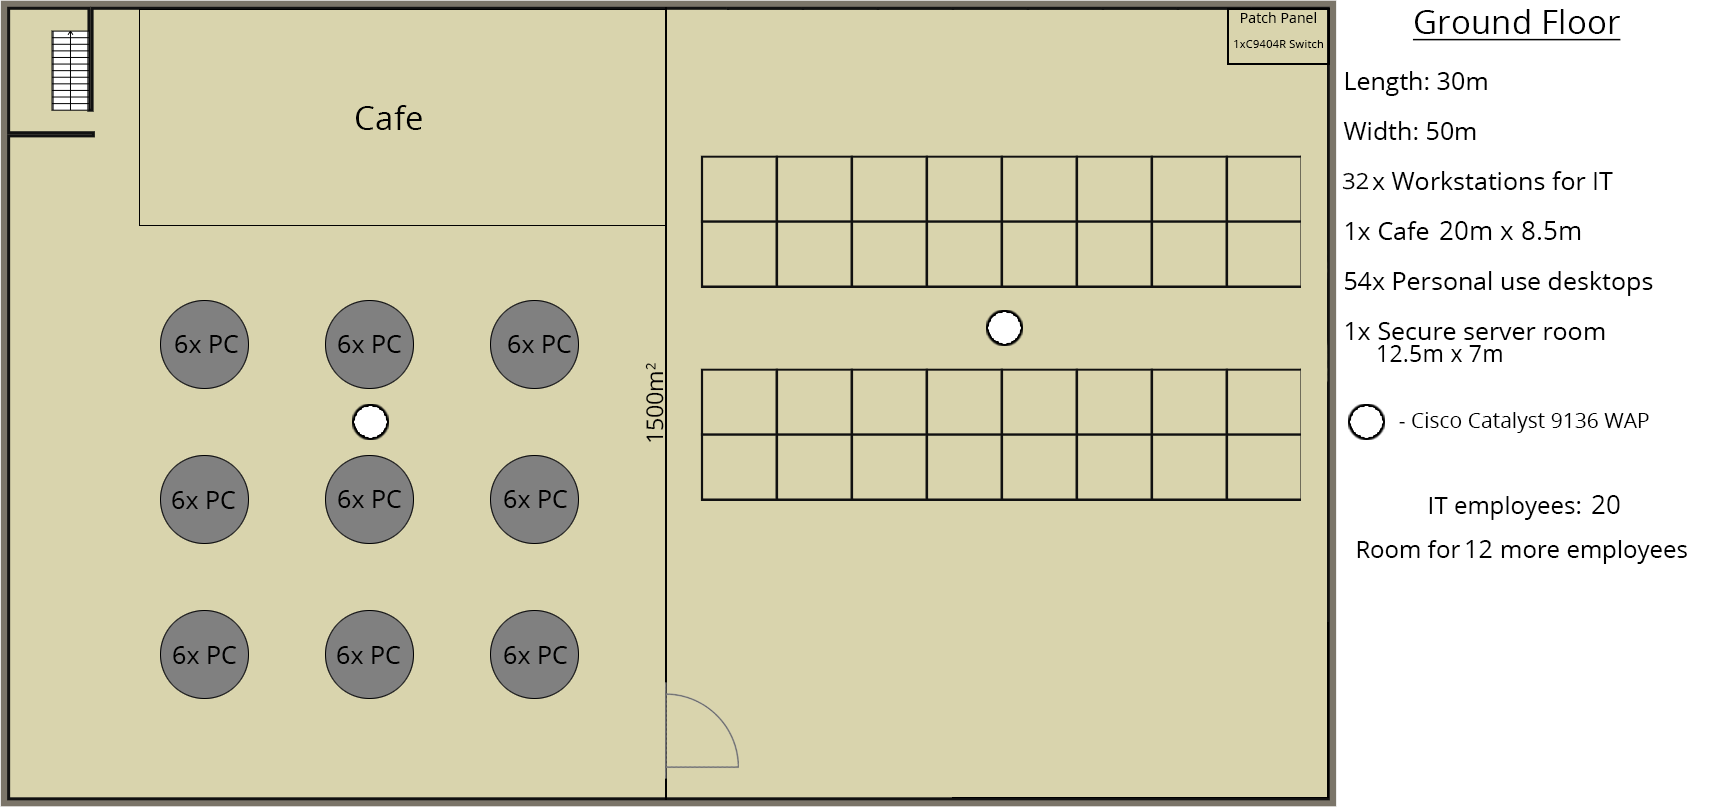
\includegraphics[width=15cm]{Figures/ground.png}
    \caption{Ground floor floor plan}
    \label{ground_floor}
\end{figure}
\subsection{1st Floor}
\begin{huge}
    MAKE NEW 1ST FLOOR
\end{huge}
\subsection{2nd Floor}
\begin{huge}
    MAKE NEW 2ND FLOOR
\end{huge}
\subsection{3rd Floor}
\begin{figure}[!h]
    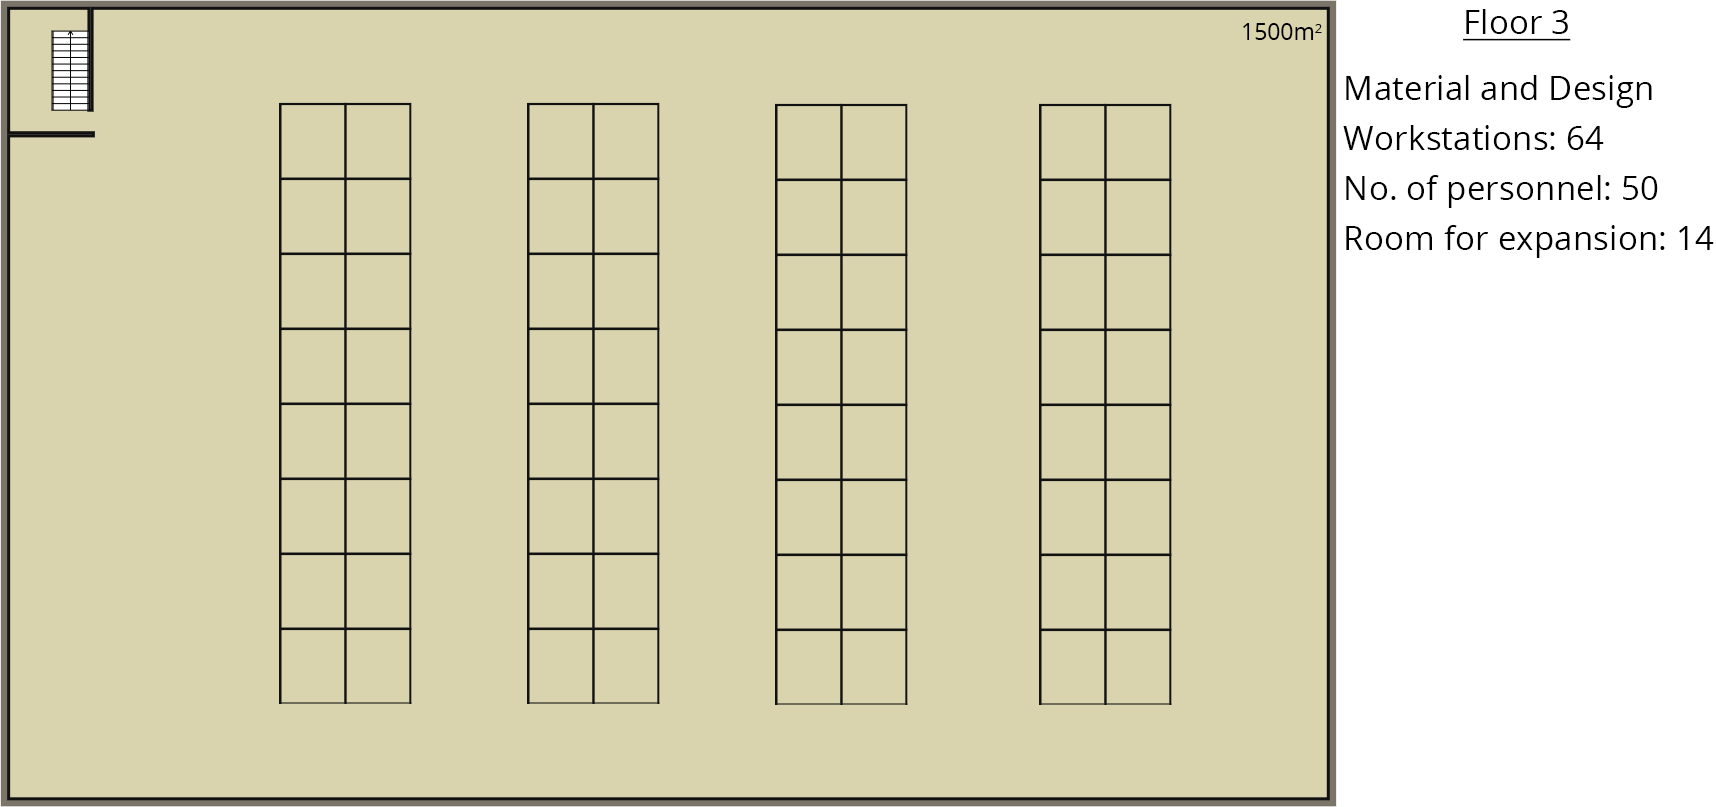
\includegraphics[width=15cm]{Figures/3rd-Floor.png}
    \caption{3rd floor floor plan}
    \label{3rd_floor}
\end{figure}
\subsection{4th Floor}
This is text
\begin{figure}[!h]
    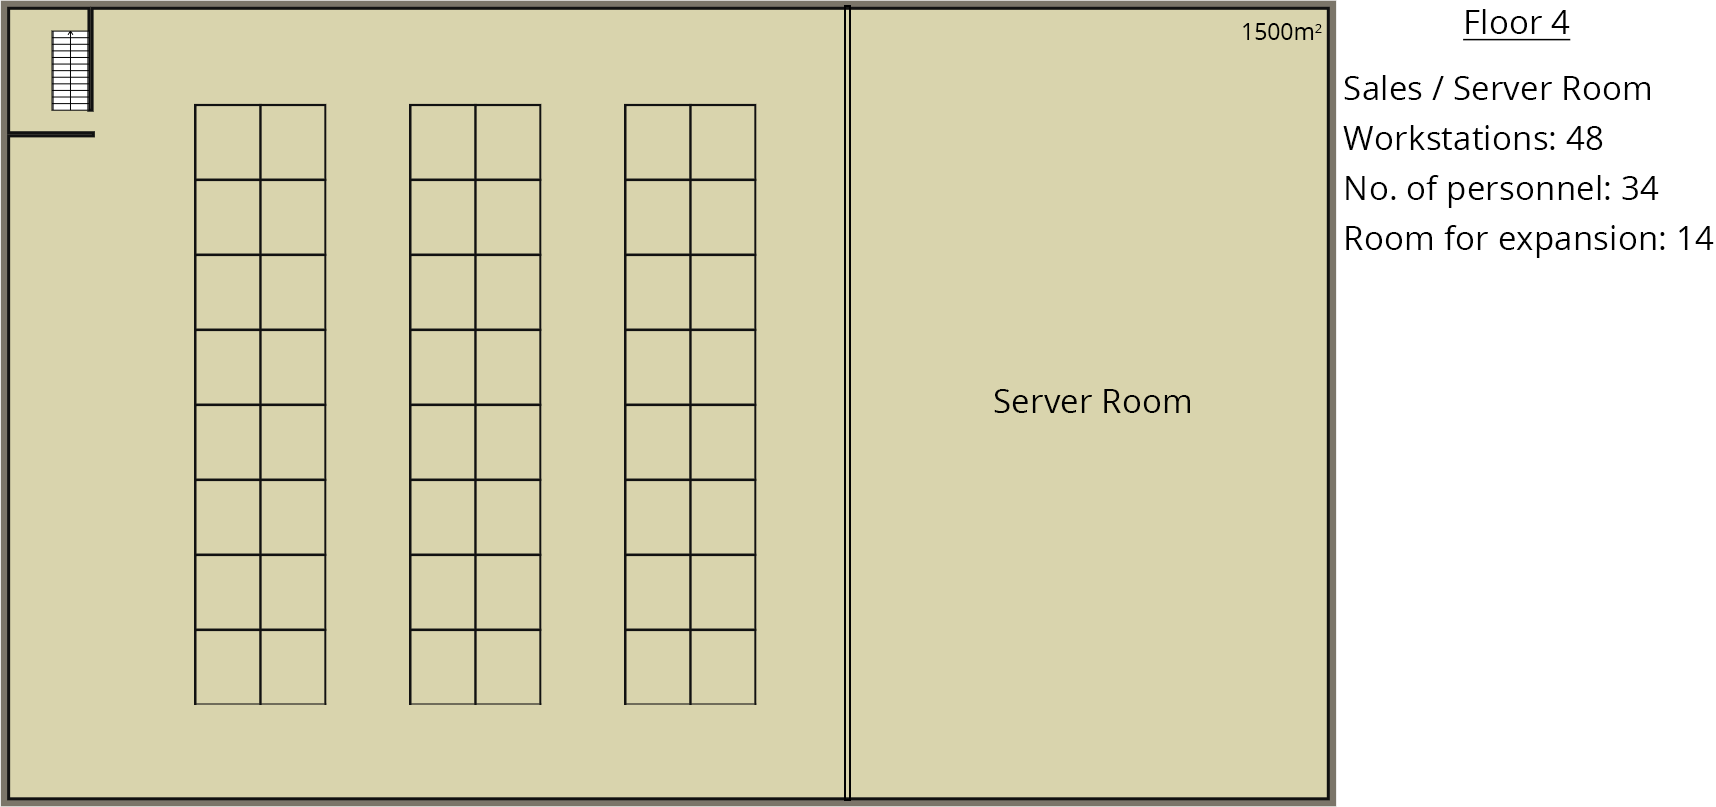
\includegraphics[width=15cm]{Figures/4th-Floor.png}
    \caption{4th floor floor plan}
    \label{4th_floor}
\end{figure}
\subsection{5th Floor}
This is text
\begin{figure}[!h]
    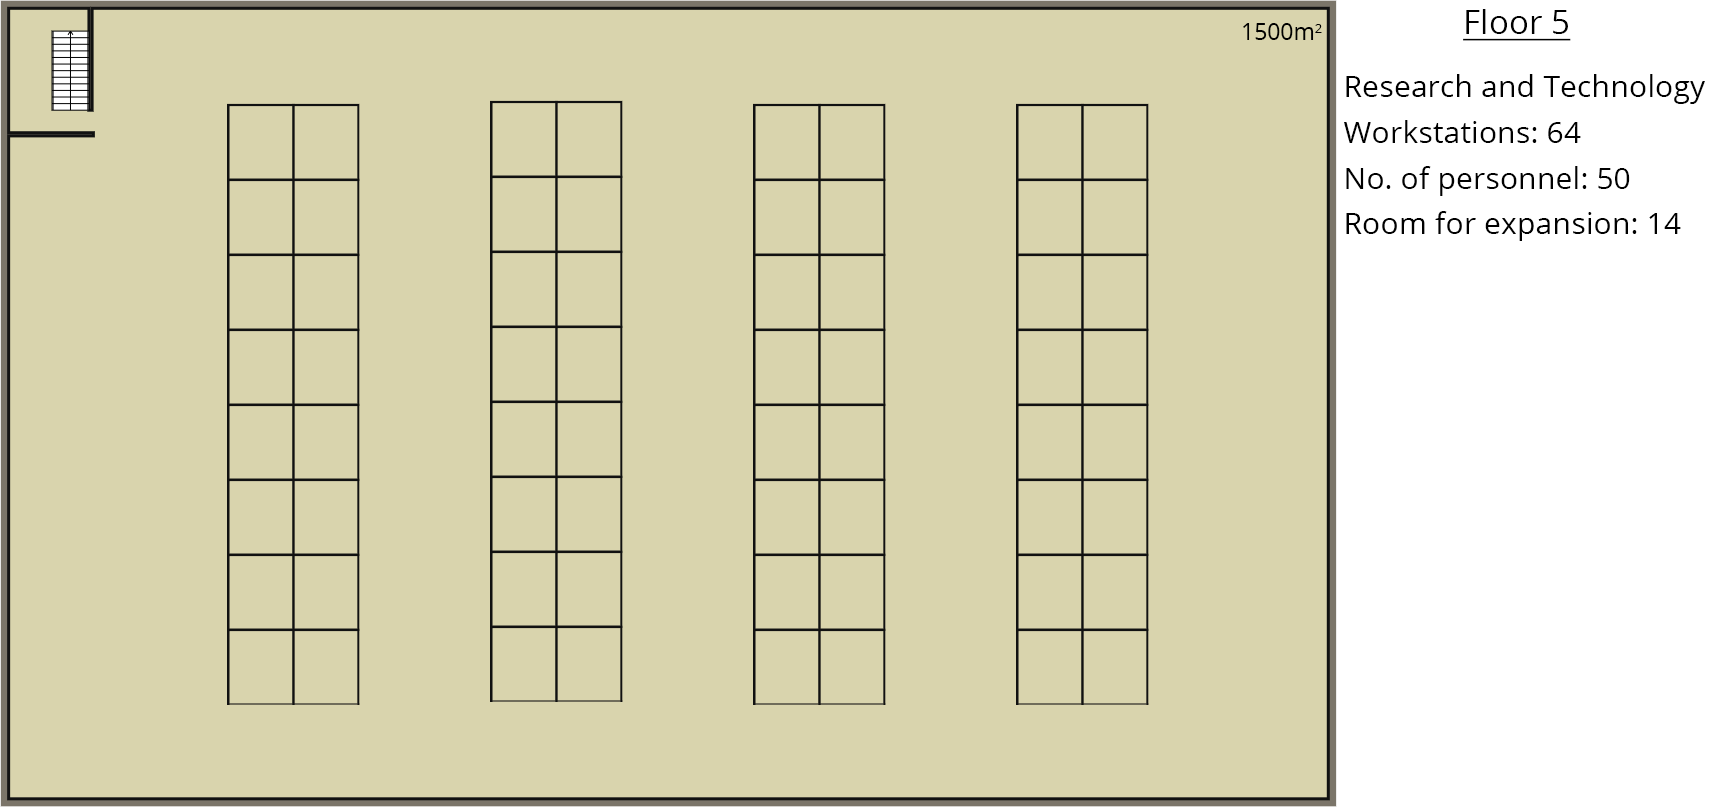
\includegraphics[width=15cm]{Figures/5th-Floor.png}
    \caption{5th floor floor plan}
    \label{5th_floor}
\end{figure}
\subsection{6th Floor}
This is text
\begin{figure}[!h]
    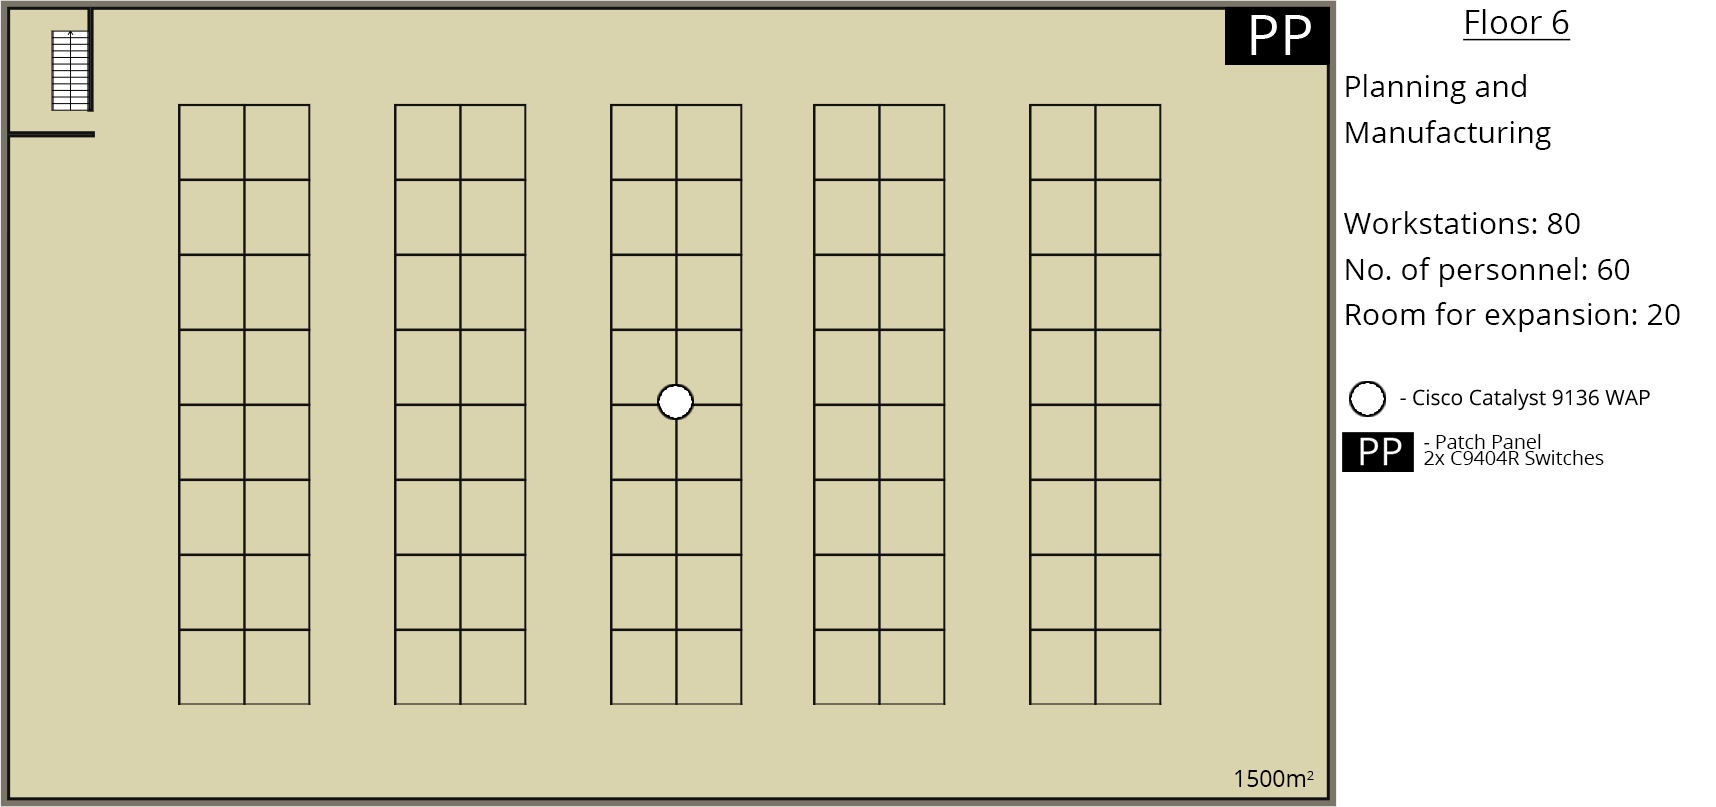
\includegraphics[width=15cm]{Figures/6th-Floor.png}
    \caption{6th floor floor plan}
    \label{6th_floor}
\end{figure}
\subsection{7th Floor}
\begin{huge}
    MAKE NEW TOP FLOOR
\end{huge}
\subsection{Server Room}